\chapter{Data Wrangling and Feature Construction}
\label{chap:wrangling}
\chapterguide
  {You should understand observations, variables, data types, and data-quality checks.}
  {select and filter records, sort data, compute grouped summaries, and create features that preserve clear meaning.}

\section{Wrangling changes representation, not the question}
Data wrangling prepares the evidence needed for analysis. Common operations are selecting variables, filtering observations, ordering records, grouping categories, aggregating summaries, joining tables, and constructing derived features.

\begin{utpfig}[Wrangling pipeline]{Each operation should be explainable as a transformation from one table to another.}{fig:wrangling-pipeline}
\begin{tikzpicture}[x=\linewidth,y=1cm,
  stage/.style={draw=UTPBlue!70,fill=UTPPaleBlue,rounded corners=1.5mm,
    line width=0.6pt,text width=0.155\linewidth,minimum height=1.55cm,
    inner xsep=1.8mm,inner ysep=2mm,align=center,
    font=\scriptsize\color{UTPNavy}},
  endpoint/.style={stage,draw=UTPTeal!80,fill=UTPPaleTeal},
  flow/.style={-{Stealth[length=2mm,width=1.5mm]},
    line width=0.8pt,draw=UTPTeal}]
\node[endpoint] (raw) at (0,0) {\textbf{Raw table}\\[4pt]
  original records\\and variables};
\node[stage] (sel) at (0.205,0) {\textbf{Select / filter}\\[4pt]
  retain relevant\\rows and columns};
\node[stage] (feat) at (0.410,0) {\textbf{Create features}\\[4pt]
  derive meaningful\\new variables};
\node[stage] (grp) at (0.615,0) {\textbf{Group / aggregate}\\[4pt]
  summarise at the\\required level};
\node[endpoint] (ana) at (0.820,0) {\textbf{Analysis table}\\[4pt]
  structured evidence\\for the question};
\draw[flow] (raw.east) -- (sel.west);
\draw[flow] (sel.east) -- (feat.west);
\draw[flow] (feat.east) -- (grp.west);
\draw[flow] (grp.east) -- (ana.west);
\end{tikzpicture}
\end{utpfig}


\section{Think in verbs: each step should have one purpose}
A readable wrangling pipeline is a sequence of simple verbs: \emph{select}, \emph{filter}, \emph{mutate}, \emph{group}, \emph{summarise}, \emph{join}, and \emph{reshape}. Keeping transformations small makes intermediate row counts and assumptions easier to audit.

\begin{utpfig}[Table transformations as contracts]{Each transformation should preserve a clear contract: what one row represents, which variables are retained, and which new values were derived.}{fig:wrangle-contract}
\begin{tikzpicture}[node distance=0.24cm,
  stage/.style={draw=UTPBlue!70,fill=UTPPaleBlue,rounded corners=1.5mm,
    line width=0.6pt,text width=0.68\linewidth,minimum height=0.90cm,
    inner xsep=3mm,inner ysep=1.5mm,align=center,
    font=\scriptsize\color{UTPNavy}},
  endpoint/.style={stage,draw=UTPTeal!80,fill=UTPPaleTeal},
  flow/.style={-{Stealth[length=1.6mm,width=1.3mm]},
    line width=0.8pt,draw=UTPTeal}]
\node[endpoint] (a) {\textbf{Input contract}\\[2pt]
  One row = one wine sample; 15 variables};
\node[stage,below=of a] (b) {\textbf{Select}\\[2pt]
  Keep cultivar, alcohol, colour intensity, and proline};
\node[stage,below=of b] (c) {\textbf{Filter}\\[2pt]
  Retain records meeting a stated inclusion rule};
\node[stage,below=of c] (d) {\textbf{Create features}\\[2pt]
  Add interpretable derived columns};
\node[endpoint,below=of d] (e) {\textbf{Output contract}\\[2pt]
  One row still = one wine sample; analysis-ready variables};
\draw[flow] (a.south) -- (b.north);
\draw[flow] (b.south) -- (c.north);
\draw[flow] (c.south) -- (d.north);
\draw[flow] (d.south) -- (e.north);
\end{tikzpicture}
\end{utpfig}

\section{Select only what the question needs}
If the question concerns alcohol, colour intensity, and cultivar, carrying every available variable into every step increases cognitive load and opportunities for mistakes.

\begin{lstlisting}[style=dsr]
analysis <- wine[, c("cultivar", "alcohol",
                     "color_intensity", "proline")]
\end{lstlisting}

\section{Filter records with explicit conditions}
Filtering defines the population being analysed. That means every filter should be stated in the report.

\begin{lstlisting}[style=dsr]
high_alcohol <- wine[wine$alcohol >= 13.5, ]
\end{lstlisting}

\begin{pitfall}
Filtering after looking at the outcome can quietly turn exploration into cherry-picking. Define inclusion rules from the analytical question or domain constraints, and disclose post-hoc filters.
\end{pitfall}


\section{Aggregation changes the unit of observation}
When rows are grouped and summarised, the output table no longer represents individual observations. One row may now represent a cultivar, region, month, or customer. This is a fundamental change in the analytical unit and should be made explicit.

\begin{utpfig}[Grouped means with uncertainty]{The cultivar means differ, while the dashed line shows the overall mean. Error bars are approximate 95\% intervals for each group mean and remind us that summaries are estimates.}{fig:wrangle-group-summary}
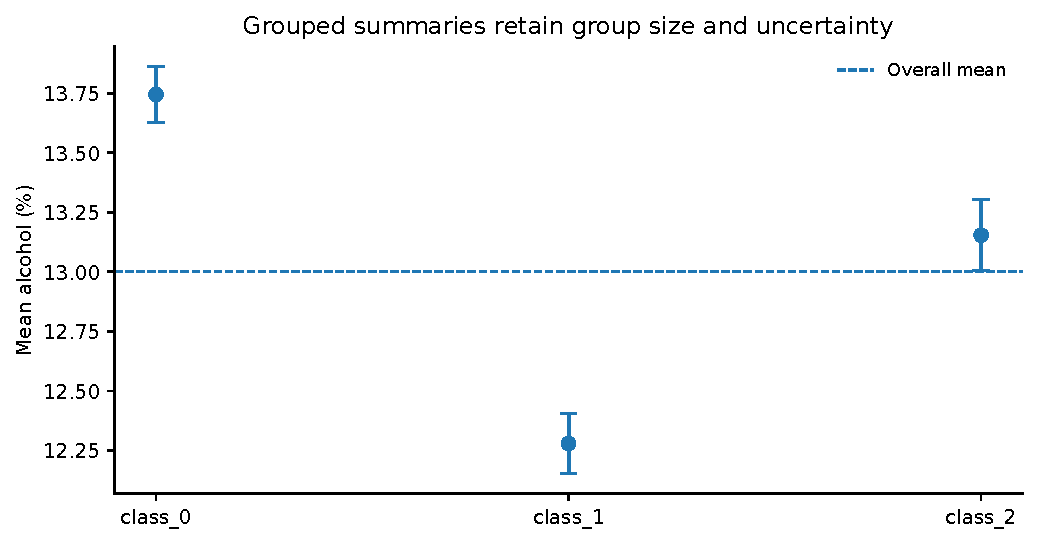
\includegraphics[width=0.80\linewidth]{figures_generated/wrangling_group_summary.pdf}
\end{utpfig}


\begin{utpfig}[A transformation changes scale and shape]{The log transformation compresses large values more strongly than small values. It can make skewed data easier to visualise or model, but it also changes coefficient interpretation.}{fig:wrangle-transform}
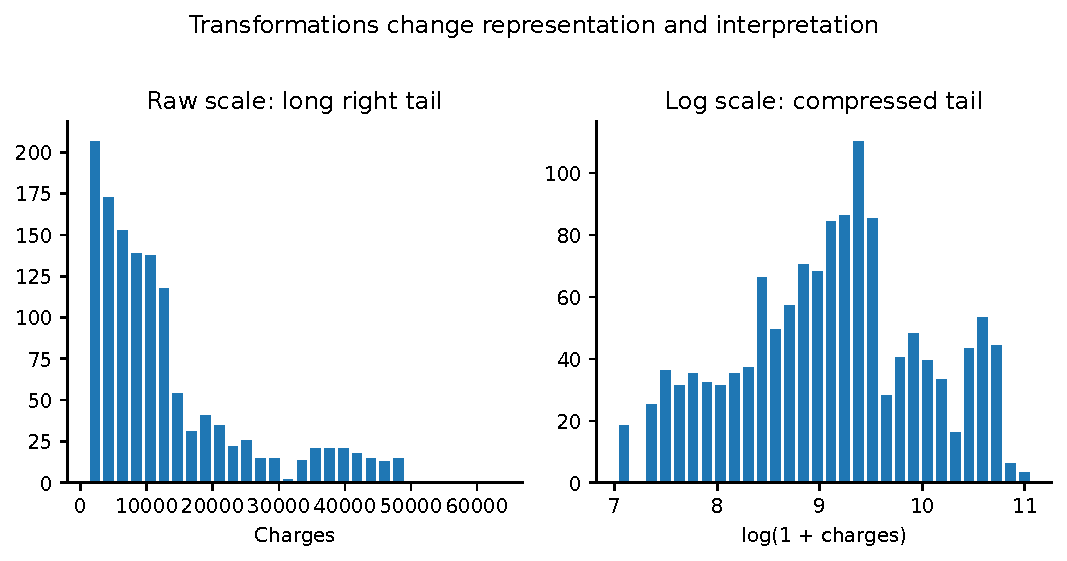
\includegraphics[width=0.82\linewidth]{figures_generated/wrangling_transform.pdf}
\end{utpfig}

\begin{keyidea}
Always ask whether a grouped result is weighted correctly for the question. Averaging three group means is not generally the same as the overall mean when group sizes differ.
\end{keyidea}

\section{Grouped summaries reveal structured differences}
Overall averages can hide subgroup structure. The \rcode{aggregate()} function makes the comparison explicit:
\begin{lstlisting}[style=dsr]
aggregate(alcohol ~ cultivar, data = wine, FUN = mean)
\end{lstlisting}
A group summary should usually include both a center and a measure of spread or sample size.


\section{Reshaping: wide and long representations}
The same information can be represented in different table shapes. \term{Wide} data often place repeated measures in separate columns, while \term{long} data place the measurement name and value in rows. Long form is often convenient for grouped plotting and repeated-measures analysis; wide form can be convenient for modelling matrices.

\begin{utpfig}[Wide and long are representations of the same information]{Reshaping should change layout, not invent or discard measurements. The key columns must be sufficient to reconstruct the original representation.}{fig:wide-long}
\begin{tikzpicture}[x=\linewidth,y=1cm,
  tablecard/.style={draw=UTPBlue!70,fill=UTPPaleBlue,rounded corners=1.5mm,
    line width=0.6pt,text width=0.38\linewidth,minimum height=3.9cm,
    inner sep=3mm,align=center,font=\scriptsize\color{UTPNavy}},
  reshape/.style={arrows={Stealth[length=2mm,width=1.5mm]-Stealth[length=2mm,width=1.5mm]},
    line width=0.8pt,draw=UTPTeal}]
% Keep the shared table defaults from enlarging these compact diagram tables.
\AtBeginEnvironment{tabular}{\scriptsize\setlength{\extrarowheight}{0pt}\rowcolors{2}{}{}}
\node[tablecard] (wide) at (0,0) {%
  \begin{minipage}[t][3.3cm][t]{\linewidth}
  \setlength{\parskip}{0pt}
  \centering
  \textbf{Wide format}\\[3pt]
  One row per ID\par\medskip
  \renewcommand{\arraystretch}{1.2}
  \setlength{\tabcolsep}{4pt}
  \begin{tabular}{@{}lrr@{}}
  \toprule
  \textbf{ID} & \textbf{temp\_morning} & \textbf{temp\_evening} \\
  \midrule
  01 & 21.4 & 26.1 \\
  02 & 20.9 & 25.6 \\
  \bottomrule
  \end{tabular}
  \end{minipage}};
\node[tablecard,draw=UTPTeal!80,fill=UTPPaleTeal] (long) at (0.55,0) {%
  \begin{minipage}[t][3.3cm][t]{\linewidth}
  \setlength{\parskip}{0pt}
  \centering
  \textbf{Long format}\\[3pt]
  One row per ID and time\par\medskip
  \renewcommand{\arraystretch}{1.2}
  \setlength{\tabcolsep}{4pt}
  \begin{tabular}{@{}llr@{}}
  \toprule
  \textbf{ID} & \textbf{time} & \textbf{temperature} \\
  \midrule
  01 & morning & 21.4 \\
  01 & evening & 26.1 \\
  02 & morning & 20.9 \\
  02 & evening & 25.6 \\
  \bottomrule
  \end{tabular}
  \end{minipage}};
\draw[reshape] (wide.east) --
  node[above=3pt,font=\scriptsize\color{UTPNavy}]{reshape}
  node[below=3pt,font=\scriptsize\color{UTPMuted}]{same values}
  (long.west);
\end{tikzpicture}
\end{utpfig}

\section{Feature engineering should add meaning}
A \term{feature} is an input variable used in analysis or modelling. New features can simplify relationships, encode domain knowledge, or make scales easier to compare.

\begin{dstable}
\begin{tabularx}{\linewidth}{@{}p{3.1cm}p{4.4cm}X@{}}
\toprule
\rowcolor{DSPaleBlue!92}
Feature operation & Example & Reason \\
\midrule
Binning & alcohol to lower/middle/higher & communicate broad ranges \\
Transformation & \(\log(1+x)\) & compress strongly right-skewed values \\
Ratio & cost per unit & represent relative rather than absolute size \\
Interaction & age \(\times\) treatment & allow one effect to vary with another \\
Indicator & missing = yes/no & preserve missingness as information \\
\bottomrule
\end{tabularx}
\end{dstable}

\begin{keyidea}
A good engineered feature has a sentence-level interpretation. If you cannot explain what the feature means without referring to the code that produced it, it is hard to defend analytically.
\end{keyidea}


\section{Join cardinality should be known before the join}
A join combines rows according to key matches. The expected relationship between keys is called \term{cardinality}. One-to-one joins should preserve row count; one-to-many joins deliberately repeat the ``one'' side; many-to-many joins can create a Cartesian multiplication and are frequently accidental.

\begin{utpfig}[Join cardinality]{Knowing the expected key relationship lets row-count changes become a diagnostic rather than a surprise.}{fig:join-cardinality}
\begin{tikzpicture}[x=\linewidth,y=1cm,
  relationship/.style={draw=UTPBlue!70,fill=UTPPaleBlue,
    rounded corners=1.5mm,line width=0.6pt,text width=0.26\linewidth,
    minimum height=2.15cm,inner xsep=2.5mm,inner ysep=2mm,
    align=center,font=\scriptsize\color{UTPNavy}},
  outcome/.style={font=\scriptsize\color{UTPMuted},align=center,
    text width=0.26\linewidth,inner sep=0pt}]
\node[relationship] (oneone) at (0,0) {\textbf{One-to-one}\\[2pt]
  \textbf{1 : 1}\\[5pt]
  One profile per ID\\One outcome per ID};
\node[relationship,draw=UTPTeal!80,fill=UTPPaleTeal] (onemany) at (0.335,0)
  {\textbf{One-to-many}\\[2pt]
   \textbf{1 : many}\\[5pt]
   One customer\\Many transactions};
\node[relationship,draw=UTPRed!80,fill=UTPPaleRed] (manymany) at (0.670,0)
  {\textbf{Many-to-many}\\[2pt]
   \textbf{many : many}\\[5pt]
   Repeated keys on both sides\\Rows can multiply};
\node[outcome,below=3mm of oneone] {Usually preserves rows};
\node[outcome,below=3mm of onemany] {Expected expansion};
\node[outcome,below=3mm of manymany,text=UTPRed!85!black]
  {\textbf{Verify carefully}};
\end{tikzpicture}
\end{utpfig}

\section{Joining tables introduces a new failure mode}
When combining tables, the join key should be unique at the expected level. A many-to-many join can multiply rows and corrupt counts.

\begin{workedexample}
Before joining customer and transaction tables, verify whether customer ID is unique in the customer table and repeated in the transaction table. That expected one-to-many relationship is part of the data model, not an implementation detail.
\end{workedexample}

\begin{quickcheck}
\begin{enumerate}
  \item Why can an overall mean be misleading when groups differ strongly?
  \item What should be stated whenever rows are filtered out?
  \item Give one reason to log-transform a feature.
  \item What join problem can cause row counts to increase unexpectedly?
\end{enumerate}
\end{quickcheck}

\section{Worked case: from 17,379 hourly rows to an interpretable demand profile}

The hourly Bike Sharing file demonstrates why wrangling is analytical work rather than clerical preparation. One row represents one observed hour. The goal is not to make the table smaller for its own sake, but to create a representation matched to a question such as ``How does the daily demand pattern differ between working and non-working days?''

\begin{utpfig}[Aggregation exposes a behavioural pattern]{A grouped hourly summary reveals commuting peaks on working days and a broader daytime pattern on non-working days. The transformation changes the grain from individual observed hours to mean demand for each hour--day-type combination.}{fig:wrangle-bike-hours}
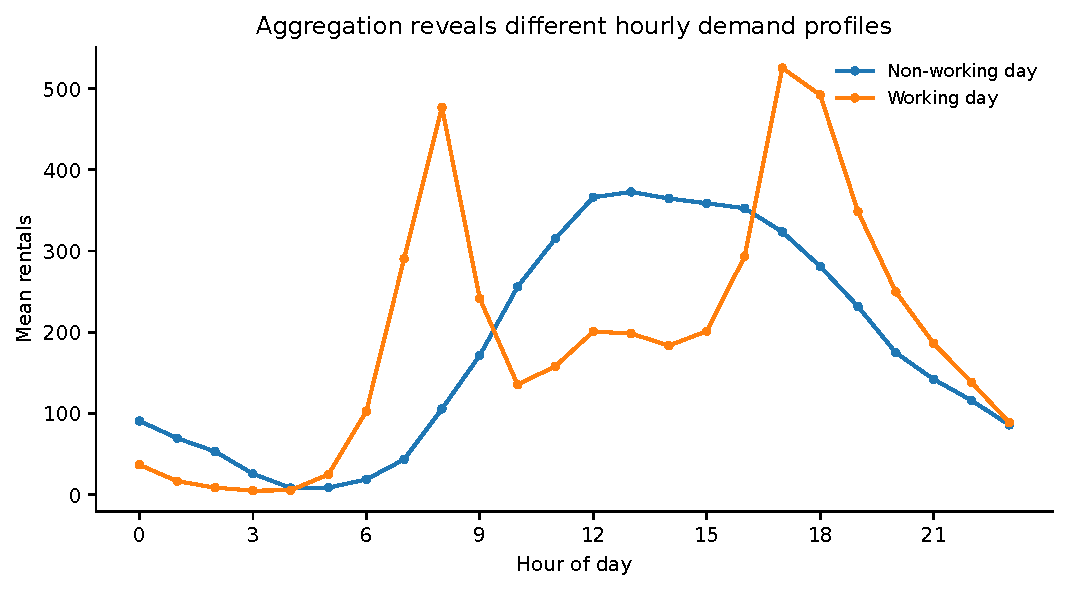
\includegraphics[width=0.86\linewidth]{figures_generated/wrangling_bike_hourly_profiles.pdf}
\end{utpfig}

A useful feature engineering detail is that clock hour is cyclical. In ordinary numeric distance, hours 23 and 0 appear 23 units apart even though they are adjacent on the clock. A common encoding maps hour to the unit circle:
\[
  h_{\sin}=\sin(2\pi h/24), \qquad h_{\cos}=\cos(2\pi h/24).
\]
This representation preserves neighbourhood around midnight and gives models two smooth numeric variables instead of an arbitrary linear scale.

\begin{keyidea}
Every aggregation changes the unit of analysis. Before and after a \rcode{group}/\rcode{summarise} operation, state what one row represents. Many subtle data errors are actually grain errors.
\end{keyidea}

\begin{chapterrecap}
\begin{itemize}
  \item Wrangling transforms tables so the evidence matches the question.
  \item Selection and filtering define the scope of analysis.
  \item Grouped summaries expose heterogeneity hidden by overall statistics.
  \item Feature engineering should be interpretable and documented.
\end{itemize}
\end{chapterrecap}
